\documentclass[12pt]{article}

\usepackage{fullpage}
\usepackage{times}
\usepackage{hyperref}
\usepackage{listings}
\usepackage{amsmath}
\usepackage{tikz}
\usetikzlibrary{automata}
\usepackage{tikz-uml}

\usepackage{amssymb}
\newcommand{\always}{\Box}
\newcommand{\eventually}{\Diamond}
\newcommand{\nxt}{\bigcirc}
\newcommand{\until}{\mathbin{\sf U}}

\newcommand{\TRUE}{\mbox{\lstinline{true}}}
\newcommand{\FALSE}{\mbox{\lstinline{false}}}
\newcommand{\NOT}{\mbox{\lstinline{!}}}
\newcommand{\AND}{\mathbin{\mbox{\lstinline{\&\&}}}}
\newcommand{\OR}{\mathbin{\mbox{\lstinline{||}}}}
\newcommand{\IMPLIES}{\mathbin{\mbox{\lstinline{->}}}}
\newcommand{\IFF}{\mathbin{\mbox{\lstinline{<->}}}}
\newcommand{\AX}{\mbox{\lstinline{AX}\,}}
\newcommand{\EX}{\mbox{\lstinline{EX}\,}}
\newcommand{\AG}{\mbox{\lstinline{AG}\,}}
\newcommand{\EG}{\mbox{\lstinline{EG}\,}}
\newcommand{\AF}{\mbox{\lstinline{AF}\,}}
\newcommand{\EF}{\mbox{\lstinline{EF}\,}}
\newcommand{\AU}{\mathbin{\mbox{\lstinline{AU}}}}
\newcommand{\EU}{\mathbin{\mbox{\lstinline{EU}}}}

\lstset{basicstyle=\ttfamily,mathescape=true}

\usepackage{amsthm}
\theoremstyle{definition}
\newtheorem{definition}{Definition}

\usepackage{stmaryrd}
\newcommand{\satisfaction}[1]{\llbracket #1 \rrbracket}

\begin{document}

\title{}
\author{}
\date{\today}
\maketitle

\section{The Syntax of Computation Tree Logic}

\emph{Computation tree logic} (CTL) was introduced by Turing award winners Clarke and Emerson \cite{CE81}.  The formulas of this logic consist of the constants \lstinline{true} and \lstinline{false} and so-called atomic propositions which are combined by means of several operators that we will discuss below.  The \emph{atomic propositions} are used to express basic facts about the states of the system.  That is, these atomic propositions are state predicates.  In the next section, we provide some concrete examples of atomic propositions in the context of Java code.

CTL contains the operators
\begin{itemize}
\item
negation, denoted $\neg$,
\item 
conjunction, denoted by $\wedge$,
\item
disjunction, denoted $\vee$,
\item
implication, denoted $\rightarrow$, and
\item
equivalence, denoted $\leftrightarrow$.
\end{itemize}
Furthermore, it contains
\begin{itemize}
\item 
universal quantification, denoted $\forall$, and
\item
existential quantification, denoted $\exists$.
\end{itemize}
Finally, it contains the so-called temporal operators
\begin{itemize}
\item 
next, denoted $\nxt$,
\item
until, denoted $\until$,
\item
always, denoted $\always$, and
\item
eventually, denoted $\eventually$.
\end{itemize}

Let us formally define the syntax of CTL.  Let $\mathit{AP}$ be the set of atomic propositions.  The set of CTL formulas is defined by the following grammar.
\begin{align*}
\varphi
::= \, & ( \varphi ) 
\mid a\\
\mid\, & \TRUE
\mid \FALSE
\mid \neg \varphi
\mid \varphi \wedge \varphi
\mid \varphi \vee \varphi
\mid \varphi \rightarrow \varphi
\mid \varphi \leftrightarrow \varphi\\
\mid \, & \forall \nxt \varphi
\mid \exists \nxt \varphi
\mid \forall \varphi \until \varphi
\mid \exists \varphi \until \varphi
\mid \forall \always \varphi
\mid \exists \always \varphi
\mid \forall \eventually \varphi
\mid \exists \eventually \varphi
\end{align*}
where $a \in \mathit{AP}$.  

In order to make sense of a CTL formula such as
\[
\forall \nxt a \rightarrow b \rightarrow c
\]
we need to define the precedence of the operators.  Furthermore, we need to specify whether the binary operators are left or right associative.  For the order of precedence, we use the commonly accepted order (from highest to lowest): $\neg$, $\wedge$, $\vee$, $\rightarrow$, and $\leftrightarrow$.  According to Baier and Katoen \cite{BK08}, $\until$ takes precedence over $\wedge$, $\vee$, and $\rightarrow$ (they do not consider $\leftrightarrow$).  Usually, unary operators have higher precedence than binary ones.  Hence, the operators, listed from highest to lowest precedence, are
\begin{align*}
& \neg\\
& \forall \nxt, \exists \nxt, \forall \always, \exists \always, \forall \eventually, \exists \eventually\\
& \forall \until, \exists \until\\
& \wedge\\
& \vee\\
& \rightarrow\\
& \leftrightarrow
\end{align*}

The binary operators $\wedge$, $\vee$ and $\leftrightarrow$ are (left) associative.  Usually, $\rightarrow$ is considered right associative.  According to Baier and Katoen \cite{BK08}, $\until$ is also right associative.

Using the above specified precedence and associativity rules, the above CTL formula is interpreted as
\[
(\forall \nxt a) \rightarrow (b \rightarrow c)
\]

To express the CTL formulas in ASCII, we use the following grammar.
\begin{align*}
\varphi
::= \, & ( \varphi ) 
\mid a\\
\mid\, & \TRUE
\mid \FALSE
\mid \NOT \varphi
\mid \varphi \AND \varphi
\mid \varphi \OR \varphi
\mid \varphi \IMPLIES \varphi
\mid \varphi \IFF \varphi\\
\mid \, & \AX \varphi
\mid \EX \varphi
\mid  \varphi \AU \varphi
\mid \varphi \EU \varphi
\mid \AG \varphi
\mid \EG \varphi
\mid \AF \varphi
\mid \EF \varphi
\end{align*}
The ASCII representation of $\neg$, $\wedge$, and $\vee$ is taken from Java.  It is common practice to use \lstinline{A} and \lstinline{E} for universal (for \emph{a}ll) and existential (\emph{e}xists) quantification.  In the seminal paper by Turing award winner Pnueli \cite{P77}, the temporal operators $\nxt$, $\until$, $\always$, and $\eventually$ are represented as \lstinline{X} (ne\emph{x}t), \lstinline{U} (\emph{u}ntil), \lstinline{G} (\emph{g}lobally), and \lstinline{F} (\emph{f}uture).  The representation of $\forall \varphi \until \varphi$ as $\varphi \AU \varphi$ is new, as far as we know.  The above CTL formula is represented in ASCII as follows.
\begin{center}
\lstinline{AX a -> b -> c}
\end{center}

\section{The Syntax of Computation Tree Logic for Java}

The next operator $\nxt$ expresses that something holds in the next state.  For Java code, if one were to define the notion of next state, it would probably be the state after the next bytecode instruction has been executed.   However, expressing properties of Java code in terms to steps taken at the bytecode level seems of limited, if any, use.  Therefore, we do not consider the next operator $\nxt$.

Recall that atomic propositions are used to express basic facts about the states.  For now, we restrict our attention to static Boolean fields.  Such an atomic proposition holds in those states in which the field has the value true.  In Java, static Boolean fields are of the form 
\begin{itemize}
\item 
$\langle$package name$\rangle$ .\ $\langle$class name$\rangle$ .\ $\langle$field name$\rangle$ or
\item
$\langle$class name$\rangle$ .\ $\langle$field name$\rangle$.
\end{itemize}
For example, the package \lstinline{java.awt} contains the classes \lstinline{AWTEvent} and \lstinline{InvocationEvent}.  The former contains the static field \lstinline{consumed} and the latter contains \lstinline{catchExceptions}.  Hence, the static Boolean field \lstinline{java.awt.AWTEvent.consumed} is an atomic proposition, as is \lstinline{java.awt.InvocationEvent.catchExceptions}.  Those fields are used as atomic propositions in the following CTL formula.
\begin{lstlisting}
AG (java.awt.AWTEvent.consumed 
    || EF !java.awt.event.InvocationEvent.catchExceptions)
\end{lstlisting}

\section{A Lexer and Parser for CTL Formulas}

A lexer and parser for CTL formulas have been developed using ANTLR \cite{P13}.  The above described grammar can be specified in ANTLR format as folows.
\begin{lstlisting}
formula
  : '(' formula ')'			#Bracket
  | ATOMIC_PROPOSITION			#AtomicProposition
  | 'true'				#True
  | 'false'				#False
  | '!' formula				#Not
  | 'AG' formula			#ForAllAlways
  | 'AF' formula			#ForAllEventually
  | 'EG' formula			#ExistsAlways
  | 'EF' formula			#ExistsEventually
  | <assoc=right> formula 'AU' formula  #ForAllUntil
  | <assoc=right> formula 'EU' formula  #ExistsUntil
  | <assoc=left> formula '&&' formula	#And
  | <assoc=left> formula '| |' formula  #Or
  | <assoc=right> formula '->' formula  #Implies
  | <assoc=left> formula '<->' formula	#Iff
\end{lstlisting}
The order of the alternatives is consistent with the precedence of the operators (if an operator has higher precedence, then its alternative occurs earlier).  The operators \lstinline{AU}, \lstinline{EU}, and \lstinline{->} are specified as right associative.  The other binary operators are left associative.  The second column of the above rule contains the labels of the alternatives (see \cite[Section~8.2]{P13}).  We will discuss their role below.

Assume that $a$, $b$, and $c$ are atomic propositions.  The formula \lstinline{$a$ AU $b$ AU $c$} is equivalent to \lstinline{$a$ AU ($b$ AU $c$)} since \lstinline{AU} is right associative.  The formula \lstinline{$a$ AU $b$ EU $c$} is equivalent to \lstinline{($a$ AU $b$) EU $c$} since \lstinline{AU} binds stronger than \lstinline{EU}.  For the same reason, the formula \lstinline{$a$ EU $b$ AU $c$} is equivalent to \lstinline{$a$ AU ($b$ EU $c$)}.

Recall that the atomic propositions are static attributes.  To specify these, we used relevant snippets of the ANTLR grammar for Java%
\footnote{See \href{https://github.com/antlr/grammars-v4/tree/master/java/java8}{github.com/antlr/grammars-v4/tree/master/java/java8}.}
Whitespace, that is, spaces, tabs, form feeds, and returns are skipped.

\textcolor{blue}{Later, we add here a discussion of error handling.}

\section{From Parse Tree to Abstract Syntax Tree}

Next, we translate a parse tree, generated by the lexer and parser, to an abstract syntax tree.  An abstract syntax tree for CTL is represented by an object of type \lstinline{Formula}, which is part of the package \lstinline{ctl}.  A UML diagram with the classes of the \lstinline{ctl} package can be found in Figure~\ref{figure:uml-abstract-syntax}.  The CTL formula
\begin{lstlisting}
AG (java.awt.AWTEvent.consumed 
    || EF !java.awt.event.InvocationEvent.catchExceptions)
\end{lstlisting}
is represented by the following \lstinline{Formula} object.
\begin{lstlisting}
Formula formula =
  new ForAllAlways(
    new Or(
      new AtomicProposition("java.awt.AWTEvent.consumed"),
      new ExistsEventually(
        new Not(
          new AtomicProposition("java.awt.event.InvocationEvent.catchExceptions")
        )
      )
    )
  );
\end{lstlisting}

\begin{figure}[ht]
\begin{center}
\begin{tikzpicture}[xscale=1.5]
\begin{umlpackage}{ctl}
    
\umlsimpleclass[type=abstract, x = 0, y = 3.5]{Formula}{}{}

\umlsimpleclass[x = 5, y = 10]{AtomicProposition}{}{}
\umlsimpleclass[x = 5, y = 9]{True}{}{}
\umlsimpleclass[x = 5, y = 8]{False}{}{}
\umlsimpleclass[x = 5, y = 7]{Not}{}{}
\umlsimpleclass[x = 5, y = 6]{And}{}{}
\umlsimpleclass[x = 5, y = 5]{Or}{}{}
\umlsimpleclass[x = 5, y = 4]{Implies}{}{}
\umlsimpleclass[x = 5, y = 3]{Iff}{}{}
\umlsimpleclass[x = 5, y = 2]{ForAllAlways}{}{}
\umlsimpleclass[x = 5, y = 1]{ForAllEventually}{}{}
\umlsimpleclass[x = 5, y = 0]{ForAllUntil}{}{}
\umlsimpleclass[x = 5, y = -1]{ExistsAlways}{}{}
\umlsimpleclass[x = 5, y = -2]{ExistsEventually}{}{}
\umlsimpleclass[x = 5, y = -3]{ExistsUntil}{}{}

\umlinherit[geometry=-|-]{Formula}{AtomicProposition}
\umlinherit[geometry=-|-]{Formula}{True}
\umlinherit[geometry=-|-]{Formula}{False}
\umlinherit[geometry=-|-]{Formula}{Not}
\umlinherit[geometry=-|-]{Formula}{And}
\umlinherit[geometry=-|-]{Formula}{Or}
\umlinherit[geometry=-|-]{Formula}{Implies}
\umlinherit[geometry=-|-]{Formula}{Iff}
\umlinherit[geometry=-|-]{Formula}{ForAllAlways}
\umlinherit[geometry=-|-]{Formula}{ForAllEventually}
\umlinherit[geometry=-|-]{Formula}{ForAllUntil}
\umlinherit[geometry=-|-]{Formula}{ExistsAlways}
\umlinherit[geometry=-|-]{Formula}{ExistsEventually}
\umlinherit[geometry=-|-]{Formula}{ExistsUntil}

\umluniaggreg[geometry=-|, mult1=1, pos1=0.8, anchor1=160]{Not}{Formula}
\umluniaggreg[geometry=-|, mult1=2, pos1=0.8, anchor1=160]{And}{Formula}
\umluniaggreg[geometry=-|, mult1=2, pos1=0.8, anchor1=160]{Or}{Formula}
\umluniaggreg[geometry=-|, mult1=2, pos1=0.8, anchor1=160]{Implies}{Formula}
\umluniaggreg[geometry=-|, mult1=2, pos1=0.8, anchor1=-160]{Iff}{Formula}
\umluniaggreg[geometry=-|, mult1=1, pos1=0.8, anchor1=-160]{ForAllAlways}{Formula}
\umluniaggreg[geometry=-|, mult1=1, pos1=0.8, anchor1=-160]{ForAllEventually}{Formula}
\umluniaggreg[geometry=-|, mult1=2, pos1=0.8, anchor1=-160]{ForAllUntil}{Formula}
\umluniaggreg[geometry=-|, mult1=1, pos1=0.8, anchor1=-160]{ExistsAlways}{Formula}
\umluniaggreg[geometry=-|, mult1=1, pos1=0.8, anchor1=-160]{ExistsEventually}{Formula}
\umluniaggreg[geometry=-|, mult1=2, pos1=0.8, anchor1=-160]{ExistsUntil}{Formula}   

\end{umlpackage}
\end{tikzpicture}
\end{center}
\caption{UML class diagram of the abstract syntax classes.}
\label{figure:uml-abstract-syntax}
\end{figure} 

To implement this translation, we use the visitor design pattern.  ANTLR supports this design pattern (see \cite[Section~7.3]{P13}).  From the CTL grammar, ANTLR generates a \lstinline{CTLVisitor} interface.  This interface contains a visit method for each alternative.  For example, for the alternative labelled \lstinline{ExistsAlways}, the interface contains the method \lstinline{visitExistsAlways}.

ANTLR also generates the \lstinline{CTLBaseVisitor} class.  This adapter class provides a default implementation for all the methods of the \lstinline{CTLVisitor} interface.  We implement our translation by extending this class and overriding methods.  For example, when we visit a node of the parse tree corresponding to the alternative labelled \lstinline{And}, we first visit the left child and obtain the \lstinline{Formula} object corresponding to the translation of the parse tree rooted at that left child.  Next, we visit the right child and obtain the \lstinline{Formula} object for the parse tree rooted at that right child.  Finally, we create an \lstinline{And} object from those two \lstinline{Formula} objects.

\begin{lstlisting}
@Override
public Formula visitAnd(AndContext context) {
  Formula left = (Formula) visit(context.formula(0));
  Formula right = (Formula) visit(context.formula(1));
  return new And(left, right);
}
\end{lstlisting}

Since the implication operator is right associative, in the \lstinline{visitImplies} method we visit the right child first.
\begin{lstlisting}
@Override
public Formula visitImplies(ImpliesContext context) {
  Formula right = (Formula) visit(context.formula(1));
  Formula left = (Formula) visit(context.formula(0));
  return new Implies(left, right);
}
\end{lstlisting}

\section{Testing the Lexer, the Parser, and the Translation}




\section{A New Semantics for CTL}

The normal semantics of CTL is described in \cite[Section~6.2.2]{BK08}.  This normal semantics is defined for a transition system $(S, Act, \rightarrow, I, AP, L)$.  Such a transition system is defined in \cite[Definition~2.1]{BK08}.  The new semantics considers a partial transition system.  A partial transition system is a tuple $(S, F, Act, \rightarrow, I, AP, L)$, where all components are defined as before and $F \subseteq S$ is a set of fully explored states.  A transition system is called partial because the states $S \setminus F$ are not fully explored yet, that is, these states have transitions that are not part of the transition relation $\rightarrow$.  

Consider the following partial transition system.
\begin{center}
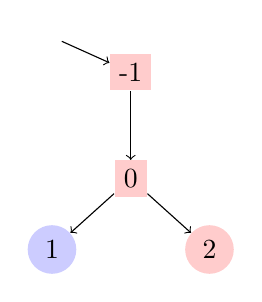
\begin{tikzpicture}[yscale=0.9]
\node (start) at (0,3) {};
\node[rectangle,fill=red!20] (-1) at (1,2.5) {-1};
\node[rectangle,fill=red!20] (0) at (1,1) {0};
\node[circle,fill=blue!20] (1) at (0,0) {1};
\node[circle,fill=red!20] (2) at (2,0) {2};

\draw[->] (start)--(-1);
\draw[->] (-1)--(0);
\draw[->] (0)--(1);
\draw[->] (0)--(2);
\end{tikzpicture}
\end{center}
State~-1 is the initial state.  The states -1 and 0 are fully explored, and  states 1 and 2 are not fully explored.  Consider, for example, the CTL formula $\exists \eventually\, \mbox{blue}$.  This formula holds in the above partial transition system, since state 1 is blue and can be reached from the initial state.  The CTL formula $\forall \always\, \mbox{red}$ does not hold for the same reason.  Now consider the CTL formula $\forall \always\, (\mbox{red} \vee \mbox{blue})$.  The above partial transition system does not provide a counterexample to this formula as all states that can be reached from the initial state are either red or blue.  However, since states 1 and 2 are not fully explored, either state may have a successor that is neither red nor blue.  So, the best we can say is ``don't know.''  Hence, whether a partial transition system satisfies a CTL formula can be answered as either yes ($\top$), no ($\perp$), or don't know (?).

Recall that the satisfaction relation $\models$, defined in \cite[Definition~6.4]{BK08}, can be viewed as mapping a state~$s$ of a transition system and a CTL formula~$\varphi$ to a Boolean, that is, $(s, \varphi)$ is mapped to true if $s \models \varphi$ and mapped to false otherwise.  The satisfaction relation $\models$ for CTL formulas on partial transition systems can be viewed as a mapping from states and formulas to $\top$, $\perp$, and ?.

We modify the definition of a transition system, as given in \cite[Definition~2.1]{BK08}, as follows.

\begin{definition}
A \emph{partial transition system} is a tuple $(S, F, \mathit{Act}, \rightarrow, I, \mathit{AP}, L)$ consisting of
\begin{itemize}
\item 
a set $S$ of \emph{states},
\item
a set $F \subseteq S$ of \emph{fully explored states},
\item
a set $\mathit{Act}$ of \emph{actions},
\item
a transition relation $\mathord{\rightarrow} \subseteq S \times \mathit{Act} \times S$,
\item
a set $I \subseteq S$ of \emph{initial states},
\item
a set $\mathit{AP}$ of \emph{atomic propositions}, and
\item
a \emph{labelling function} $L : S \to 2^{\mathit{AP}}$.
\end{itemize}
\end{definition}

The difference between a partial transition system and an ordinary transition system is the set $F$ of fully explored states.  Since the set $\mathit{Act}$ of actions does not play in the remainder, we will drop it from the definition and simplify the transition relation to $\mathord{\rightarrow} \subseteq S \times S$. The partial transition system depicted in the introduction can be formally defined as $(S, F, \rightarrow, I, \mathit{AP}, L)$ where
\begin{itemize}
\item 
$S = \{ -1, 0, 1, 2 \}$,
\item
$F = \{ -1, 0 \}$,
\item
$\mathord{\rightarrow} = \{ (-1, 0), (0, 1), (0, 2) \}$,
\item
$I = \{ -1 \}$,
\item
$\mathit{AP} = \{ \mbox{blue}, \mbox{red} \}$, and
\item
and the function $L : S \to 2^{\mathit{AP}}$ is defined by
\begin{align*}
L(-1) & = \{ \mbox{red} \}\\
L(0) & = \{ \mbox{red} \}\\
L(1) & = \{ \mbox{blue} \}\\
L(2) & = \{ \mbox{red} \}
\end{align*}
\end{itemize} 

\textcolor{blue}{We may have to redefine paths.}

The satisfaction relation $\models$ for CTL for ordinary transition systems is defined in \cite[Definition~6.4]{BK08}.  It can be viewed as a function $\satisfaction{\ }$ that maps each CTL formula and state of a transition system to either true of false, that is, for each state formula $\varphi$ and state $s$,
\[
s \models \varphi \mbox{ iff } \satisfaction{\varphi}(s) = \mbox{true}.
\]

To deal with partial transition systems, we extend the range of the function $\satisfaction{\ }$.  Given a formula $\varphi$ and a state $s$, we have that either
\begin{itemize}
\item 
$\satisfaction{\varphi}(s) = \top$: the formula $\varphi$ holds in the state $s$,
\item
$\satisfaction{\varphi}(s) = \perp$: the formula $\varphi$ does not hold in the state $s$, or
\item
$\satisfaction{\varphi}(s) = \mathord{?}$: we cannot determine whether the formula $\varphi$ holds in the state $s$ since some states, relevant to $\varphi$,  have not been explored.
\end{itemize}

For example, consider the partial transition system depicted above.  Consider the formula $\forall \nxt \mbox{red}$.  We have that $\satisfaction{\forall \nxt \mbox{red}}(-1) = \top$ since the state $-1$ is fully explored and all its successor states are red.  Furthermore, $\satisfaction{\forall \nxt \mbox{red}}(0) = \perp$ since one of the  successor states of state 0 is not red.  Finally, $\satisfaction{\forall \nxt \mbox{red}}(1) = \mathord{?}$ since the state 1 is not fully explored and it does not have a successor that is not red.

We denote the set of three values, $\top$, $\perp$ and $?$ by $\mathbb{V}$, that is,
\[
\mathbb{V} = \{ \top, \perp, \mathord{?} \}.
\]
We can extend the usual Boolean operators to $\mathbb{V}$ as follows.  Negation is captured in the following table.
\[
\begin{array}{c|c}
v & \neg v\\\hline
\top & \perp\\
\perp & \top\\
\mathord{?} & \mathord{?}
\end{array}
\]
Conjunction is defined as follows.
\[
\begin{array}{cc|ccc}
\multicolumn{2}{c|}{v \wedge w} & & w &\\
&& \top & \perp & \mathord{?}\\\hline
& \top & \top & \perp & \mathord{?}\\
v & \perp & \perp & \perp & \perp\\
& \mathord{?} & \mathord{?} & \perp & \mathord{?}
\end{array}
\]
Disjunction is defined as follows.
\[
\begin{array}{cc|ccc}
\multicolumn{2}{c|}{v \vee w} & & w &\\
&& \top & \perp & \mathord{?}\\\hline
& \top & \top & \top & \top\\
v & \perp & \top & \perp & \mathord{?}\\
& \mathord{?} & \top & \mathord{?} & \mathord{?}
\end{array}
\]
Implication is defined as follows.
\[
\begin{array}{cc|ccc}
\multicolumn{2}{c|}{v \rightarrow w} & & w &\\
&& \top & \perp & \mathord{?}\\\hline
& \top &  &  & \\
v & \perp &  &  & \\
& \mathord{?} &  &  & 
\end{array}
\]
Equivalence is defined as follows.
\[
\begin{array}{cc|ccc}
\multicolumn{2}{c|}{v \leftrightarrow w} & & w &\\
&& \top & \perp & \mathord{?}\\\hline
& \top &  &  & \\
v & \perp &  &  & \\
& \mathord{?} &  &  & 
\end{array}
\]

We denote the set of CTL formulas by $\mathit{CTL}$.

\begin{definition}
Let $(S, F, \rightarrow, I, \mathit{AP}, L)$ be a partial transition system.  Let $s \in S$.  The function 
\[
\satisfaction{\ } : \mathit{CTL} \to S \to \mathbb{V}
\] 
is defined by structural induction on the CTL formula as follows.
\begin{itemize}
\item
$\satisfaction{a}(s) = 
\left \{
\begin{array}{ll}
\top & \mbox{if $a \in L(s)$}\\
\perp & \mbox{otherwise}
\end{array}
\right.$
\item 
$\satisfaction{\TRUE}(s) = \top$
\item 
$\satisfaction{\FALSE}(s) = \perp$
\item
$\satisfaction{\neg \varphi}(s) = \neg \satisfaction{\varphi}(s)$
\item
$\satisfaction{\varphi \wedge \psi}(s) = \satisfaction{\varphi}(s) \wedge  \satisfaction{\psi}(s)$
\item
$\satisfaction{\varphi \vee \psi}(s) = \satisfaction{\varphi}(s) \vee  \satisfaction{\psi}(s)$
\item
$\satisfaction{\varphi \rightarrow \psi}(s) = \satisfaction{\varphi}(s) \rightarrow  \satisfaction{\psi}(s)$
\item
$\satisfaction{\varphi \leftrightarrow \psi}(s) = \satisfaction{\varphi}(s) \leftrightarrow  \satisfaction{\psi}(s)$
\item
$\satisfaction{\forall \nxt \varphi}(s) = $
\item
$\satisfaction{\exists \nxt \varphi}(s) = $
\item
$\satisfaction{\forall \varphi \until \psi}(s) = $
\item
$\satisfaction{\exists \varphi \until \psi}(s) = $
\item
$\satisfaction{\forall \always \varphi}(s) = $
\item
$\satisfaction{\exists \always \varphi}(s) = $
\item
$\satisfaction{\forall \eventually \varphi}(s) = $
\item
$\satisfaction{\exists \eventually \varphi}(s) = $
\end{itemize}
\end{definition}

\section{JPF Listener that Writes a Partial Transition System to File}

The first objective of this project is to develop a listener for Java PathFinder (JPF) that writes its partial transition system to file.  In \cite[Section~7.3]{B20}, a listener that writes a transition system to file has been developed.  This listener is extended to the setting of partial transition systems.

Consider the following partial transition system.
\begin{center}
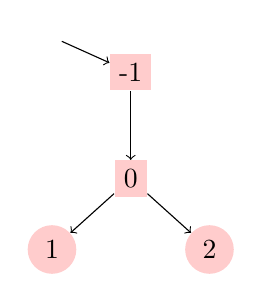
\begin{tikzpicture}[yscale=0.9]
\node (start) at (0,3) {};
\node[rectangle,fill=red!20] (-1) at (1,2.5) {-1};
\node[rectangle,fill=red!20] (0) at (1,1) {0};
\node[circle,fill=red!20] (1) at (0,0) {1};
\node[circle,fill=red!20] (2) at (2,0) {2};

\draw[->] (start)--(-1);
\draw[->] (-1)--(0);
\draw[->] (0)--(1);
\draw[->] (0)--(2);
\end{tikzpicture}
\end{center}
State~-1 is the initial state.  The states -1 and 0 are fully explored, and  states 1 and 2 are not fully explored.  The listener produces a file, the name of which is the name of the system under test with ``.tra'' as suffix (see \cite[Section 7.4]{B20}), with the following content.
\begin{verbatim}
-1 0
0 1
0 2
-1 0
\end{verbatim}
The first three lines describe the transitions.  Each line contains the source of the transition followed by the target of the transition.  The last line contains the states that are fully explored.

\bibliographystyle{plain}
\bibliography{report}

\end{document}

%
%\section{Normal forms for CTL}
%
%\description
%The objective of this project is to develop a translation of CTL formulas to equivalent formulas in existential normal form and positive normal form for partial transition systems (as defined in the ``new semantics for CTL'' project).  Existential normal form is introduced in Definition~6.13 of the textbook and positive normal form is defined in Definition~6.15.  These normal forms may have to be adjusted to deal with partial transition systems.  
%
%\resources
%\begin{itemize}
%\item 
%The textbook.
%\end{itemize}
%
%\deliverables
%\begin{itemize}
%\item
%Definitions of existential normal form and positive normal form for CTL for partial transition systems.
%\item
%A proof that for each CTL formula there exists an equivalent CTL formula in existential normal form in the context of partial transition systems (similar to the proof of Theorem~6.14 of the textbook, but considering partial transition systems and providing more details).  A similar result for positive normal form (see Theorem~6.16 of the textbook).
%\item
%A report containing the definitions, the proofs, and several examples illustrating how CTL formulas are translated into the normal forms.
%\end{itemize}
%
%\section{Translation of CTL to normal forms}
%
%\description
%The objective of this project is to implement the translation of CTL to both normal forms developed in the "normal forms for CTL" project. 
%
%Implement a class named \lstinline{ExistentialNormalForm} that contains a static method named \lstinline{translate}.  This method takes as argument an object of type \lstinline{Formula}, which is part of the \lstinline{ctl} package.  The API of the \lstinline{ctl} package can be found \href{https://www.eecs.yorku.ca/course_archive/2020-21/W/4315/project/api/ast}{here} and has been implemented in the ``from parse tree to abstract syntax tree'' project.  Similarly, develop a class named \lstinline{PositiveNormalForm} that contains a static method named \lstinline{translate}.
%
%To represent a CTL formula in the normal forms, you may use classes of the \lstinline{ctl} package.  You may also add new classes to this package.  A CTL formula can be translated to its existential normal form as follows.
%\begin{lstlisting}
%Formula formula = ...
%Formula normalForm = ExistentialNormalForm.translate(formula);
%\end{lstlisting}
%
%\deliverables
%\begin{itemize}
%\item
%Properly documented Java code that implements both translations of CTL to the normal forms.
%\item
%A test suite, using JUnit, that rigorously tests the translations.
%\item
%A report describing the design, implementation, and testing of the translations.
%\end{itemize}
%
%
%\section{CTL model checking algorithm for partial transition systems}
%
%\description
%The objective of this project is to adjust the CTL model checking algorithm, as described in Section~6.4.1 of the textbook, to the setting of partial transition systems, as developed in the ``new semantics for CTL'' project.  Given a partial transition system and a CTL formula in existential normal form, as developed in the `` existential normal form for CTL'' project, the algorithm computes the corresponding satisfaction set.
%
%\resources
%\begin{itemize}
%\item 
%The textbook.
%\end{itemize}
%
%\deliverables
%\begin{itemize}
%\item 
%An algorithm, similar to Algorithm~14 of the textbook, for the computation of the satisfaction sets of CTL formulas in existential normal form for a partial transition system.
%\item
%A proof that proves the algorithm is correct, similar to Theorem~6.23 of the textbook.
%\item
%A report describing the algorithm and its correctness proof.
%\end{itemize}
%
%\section{JPF listener that writes a partial transition system to file}
%
%\description
%The first objective of this project is to develop a listener for Java PathFinder (JPF) that writes its partial transition system to file.  Partial transition systems are defined in the ``new semantics for CTL'' project.  In Section~7.3 of the notes, a listener that writes a transition system to file has been developed.  This listener needs to be extended to the setting of partial transition systems.
%
%Consider the following partial transition system.
%\begin{center}
%\begin{tikzpicture}[yscale=0.9]
%\node (start) at (0,3) {};
%\node[rectangle,fill=red!20] (-1) at (1,2.5) {-1};
%\node[rectangle,fill=red!20] (0) at (1,1) {0};
%\node[circle,fill=red!20] (1) at (0,0) {1};
%\node[circle,fill=red!20] (2) at (2,0) {2};
%
%\draw[->] (start)--(-1);
%\draw[->] (-1)--(0);
%\draw[->] (0)--(1);
%\draw[->] (0)--(2);
%\end{tikzpicture}
%\end{center}
%State~-1 is the initial state.  The states -1 and 0 are fully explored, and  states 1 and 2 are not fully explored.  The listener should produce a file, the name of which is the name of the system under test with ``.tra'' as suffix (see Section 7.4 of the notes), with the following content.
%\begin{verbatim}
%-1 -> 0
%0 -> 1
%0 -> 2
%1 2
%\end{verbatim}
%The first three lines describe the transitions.  The last line contains the states that are not fully explored.
%
%The second objective of this project is to develop a listener for JPF that writes a graphical representation, using the DOT format, of a partial transition system to file.  In Section~7.4 of the notes, a similar listener is described.
%
%\resources
%\begin{itemize}
%\item 
%\href{https://wiki.eecs.yorku.ca/course_archive/2019-20/W/4315/_media/notes.pdf}{Java PathFinder: a tool to detect bugs in Java code}.
%\item
%\href{https://github.com/javapathfinder/jpf-core/wiki}{The Java PathFinder website}.
%\end{itemize}
%
%\deliverables
%\begin{itemize}
%\item 
%Properly documented Java code of the listeners.
%\item
%A test suite, ideally using JPF's extension of JUnit, that rigorously tests the listeners.
%\item
%A report describing the design, implementation, and testing of the listeners.
%\end{itemize}
%
%\section{Implementation of CTL model checking algorithm}
%
%\description
%The main objective of this project is to implement the algorithm developed in the ``CTL model checking algorithm for partial transition systems'' project.  As input, the algorithm takes a CTL formula in existential normal form, as implemented in the ``translation of CTL to existential normal form,'' and a partial transition system, provided by the `` JPF listener that writes a partial transition system to file.'' Another objective of this project is to design a simple GUI to import the file containing the partial transition system, to enter the CTL formula, and to run the implemented algorithm.
%
%\resources
%\begin{itemize}
%\item
%The textbook.
%\end{itemize}
%
%\deliverables
%\begin{itemize}
%\item 
%Properly documented Java code that implements the algorithm and the GUI.
%\item
%A test suite, using JUnit, that rigorously tests the implementation of the algorithm.
%\item
%A report describing the design, implementation, and testing of the algorithm.
%\end{itemize}
%
%\section{Dependencies between the projects}
%
%Several projects depend on other projects.  The diagram below depicts these dependencies.  If there is an arrow from one project to another, it means that the latter is dependent on the former.  As a consequence, the latter project needs (some of) the results of the former project.
%
%\begin{center}
%\begin{tikzpicture}
%\node (1) at (0,4) {1};
%\node (2) at (0,3) {2};
%\node (3) at (2,4) {3};
%\node (4) at (2,3) {4};
%\node (5) at (1,2) {5};
%\node (6) at (3,2) {6};
%\node (7) at (5,2) {7};
%\node (8) at (3,1) {8};
%
%\draw[->] (1)--(2);
%\draw[->] (2)--(5);
%\draw[->] (3)--(4);
%\draw[->] (4)--(5);
%\draw[->] (4)--(6);
%\draw[->] (5)--(8);
%\draw[->] (6)--(8);
%\draw[->] (7)--(8);
%\end{tikzpicture}
%\end{center}
%
%Because of these dependencies, deadlines of the projects differ.
%
%\begin{tabular}{rl}
%project number & deadline\\
%\hline
%1 & March 5\\
%2 & March 26\\
%3 & March 5\\
%4 & March 26\\
%5 & April 9\\
%6 & April 9\\
%7 & April 9\\
%8 & April 23 
%\end{tabular}
%
%\end{document}